%%%%%%%%%%%%%%%%%%%%%%%%%%%%%%%%%%%%%%%%%
% Programming/Coding Assignment
% LaTeX Template
%
% This template has been downloaded from:
% http://www.latextemplates.com
%
% Original author:
% Ted Pavlic (http://www.tedpavlic.com)
%
% Note:
% The \lipsum[#] commands throughout this template generate dummy text
% to fill the template out. These commands should all be removed when 
% writing assignment content.
%
% This template uses a Perl script as an example snippet of code,
% most other languages are also usable. Configure them in the
% "CODE INCLUSION CONFIGURATION" section.
%%%%%%%%%%%%%%%%%%%%%%%%%%%%%%%%%%%%%%%%%

%-------------------------------------------------------------------------
%	PACKAGES AND OTHER DOCUMENT CONFIGURATIONS
%-------------------------------------------------------------------------

\documentclass{article}

\usepackage{fancyhdr} % Required for custom headers
\usepackage{lastpage} % Required to determine the last page for the footer
\usepackage{extramarks} % Required for headers and footers
\usepackage[usenames,dvipsnames]{color} % Required for custom colors
\usepackage{graphicx} % Required to insert images
\usepackage{listings} % Required for insertion of code
\usepackage{courier} % Required for the courier font
\usepackage{hyperref}
\usepackage{amsmath}
\usepackage{bm}
\usepackage{mathrsfs}
\usepackage{float}
\usepackage{enumitem}
\usepackage[english]{babel}
\usepackage[utf8]{inputenc}
\usepackage{fontenc}
\usepackage{booktabs}
\usepackage{pdfpages}
% Margins
\topmargin=-0.45in
\evensidemargin=0in
\oddsidemargin=0in
\textwidth=6.5in
\textheight=9.0in
\headsep=0.25in

\linespread{1.1} % Line spacing

% Set up the header and footer
\pagestyle{fancy}
\lhead{\hmwkAuthorName} % Top left header
\chead{\hmwkClassShort\ (\hmwkClassInstructor)} % Top center head
%\rhead{\firstxmark} % Top right header
\rhead{\hmwkTitle}
\lfoot{\lastxmark} % Bottom left footer
\cfoot{} % Bottom center footer
% Bottom right footer
\rfoot{Page\ \thepage\ of\ \protect\pageref{LastPage}} 
\renewcommand\headrulewidth{0.4pt} % Size of the header rule
\renewcommand\footrulewidth{0.4pt} % Size of the footer rule

\setlength\parindent{0pt} % Removes all indentation from paragraphs

%--------------------------------------------------------------------------
%	CODE INCLUSION CONFIGURATION
%--------------------------------------------------------------------------
% This is the color used for comments
\definecolor{MyDarkGreen}{rgb}{0.0,0.4,0.0} 
\lstloadlanguages{Perl,Python} % Load Perl syntax for listings,
% for a list of other languages supported see:
%ftp://ftp.tex.ac.uk/tex-archive/macros/latex/contrib/listings/listings.pdf
\lstset{language=Perl, % Use Perl in this example
        frame=single, % Single frame around code
        basicstyle=\small\ttfamily, % Use small true type font
        keywordstyle=[1]\color{Blue}\bf, % Perl functions bold and blue
        keywordstyle=[2]\color{Purple}, % Perl function arguments purple
        % Custom functions underlined and blue
        keywordstyle=[3]\color{Blue}\underbar, 
        identifierstyle=, % Nothing special about identifiers
        % Comments small dark green courier font
        commentstyle=\usefont{T1}{pcr}{m}{sl}\color{MyDarkGreen}\small, 
        stringstyle=\color{Purple}, % Strings are purple
        showstringspaces=false, % Don't put marks in string spaces
        tabsize=5, % 5 spaces per tab
        %
        % Put standard Perl functions not included
        % in the default language here
        morekeywords={rand},
        %
        % Put Perl function parameters here
        morekeywords=[2]{on, off, interp},
        %
        % Put user defined functions here
        morekeywords=[3]{test},
       	%
        % Line continuation (...) like blue comment
        morecomment=[l][\color{Blue}]{...}, 
        numbers=left, % Line numbers on left
        firstnumber=1, % Line numbers start with line 1
        numberstyle=\tiny\color{Blue}, % Line numbers are blue and small
        stepnumber=5 % Line numbers go in steps of 5
}


\lstset{language=Python, % Use Python in this example
        frame=single, % Single frame around code
        basicstyle=\small\ttfamily, % Use small true type font
        keywordstyle=[1]\color{Blue}\bf, % Python functions bold and blue
        keywordstyle=[2]\color{Purple}, % Python function arguments purple
        % Custom functions underlined and blue
        keywordstyle=[3]\color{Blue}\underbar, 
        identifierstyle=, % Nothing special about identifiers
        % Comments small dark green courier font
        commentstyle=\usefont{T1}{pcr}{m}{sl}\color{MyDarkGreen}\small, 
        stringstyle=\color{Purple}, % Strings are purple
        showstringspaces=false, % Don't put marks in string spaces
        tabsize=3, % 5 spaces per tab
        %
        % Put standard Python functions not included in the
        % default language here
        morekeywords={rand},
        %
        % Put Python function parameters here
        morekeywords=[2]{on, off, interp},
        %
        % Put user defined functions here
        morekeywords=[3]{test},
       	%
        % Line continuation (...) like blue comment
        morecomment=[l][\color{Blue}]{...}, 
        numbers=left, % Line numbers on left
        firstnumber=1, % Line numbers start with line 1
        numberstyle=\tiny\color{Blue}, % Line numbers are blue and small
        stepnumber=5 % Line numbers go in steps of 5
}


% Creates a new command to include a perl script, the first
% parameter is the filename of the script (without .pl), the
% second parameter is the caption
\newcommand{\perlscript}[2]{
\begin{itemize}
\item[]\lstinputlisting[caption=#2,label=#1]{#1.pl}
\end{itemize}
}
\newcommand{\pythonscript}[2]{
\begin{itemize}
\item[]\lstinputlisting[caption=#2,label=#1]{#1}
\end{itemize}
}
\newcommand{\tss}{\textsuperscript}
\newcommand{\tsbs}{\textsubscript}

%--------------------------------------------------------------------------
%	DOCUMENT STRUCTURE COMMANDS
%	Skip this unless you know what you're doing
%--------------------------------------------------------------------------

% Header and footer for when a page split occurs within a
% problem environment
\newcommand{\enterProblemHeader}[1]{
\nobreak\extramarks{#1}{#1 continued on next page\ldots}\nobreak
\nobreak\extramarks{#1 (continued)}{#1 continued on next page\ldots}\nobreak
}

% Header and footer for when a page split occurs between problem
% environments
\newcommand{\exitProblemHeader}[1]{
\nobreak\extramarks{#1 (continued)}{#1 continued on next page\ldots}\nobreak
\nobreak\extramarks{#1}{}\nobreak
}

\setcounter{secnumdepth}{0} % Removes default section numbers
% Creates a counter to keep track of the number of problems
\newcounter{homeworkProblemCounter} 

\newcommand{\homeworkProblemName}{}
\newenvironment{homeworkProblem}[1][Problem \arabic{homeworkProblemCounter}]{ % Makes a new environment called homeworkProblem which takes
   % 1 argument (custom name) but the default is "Problem #"
  % Increase counter for number of problems
  \stepcounter{homeworkProblemCounter}
  % Assign \homeworkProblemName the name of the problem
  \renewcommand{\homeworkProblemName}{#1}
  % Make a section in the document with the custom problem count
  \section{\homeworkProblemName}
  % Header and footer within the environment  
  \enterProblemHeader{\homeworkProblemName} 
}{
  % Header and footer after the environment
  \exitProblemHeader{\homeworkProblemName}
}
% Defines the problem answer command with the content as the only argument
 % Makes the box around the problem answer and puts the content inside
\newcommand{\problemAnswer}[1]{ 
\noindent\framebox[\columnwidth][c]{\begin{minipage}{0.98\columnwidth}#1\end{minipage}}
}

\newcommand{\homeworkSectionName}{}
\newenvironment{homeworkSection}[1]{ % New environment for sections within homework problems, takes 1 argument - the name of the section
\renewcommand{\homeworkSectionName}{#1} % Assign \homeworkSectionName to the name of the section from the environment argument
\subsection{\homeworkSectionName} % Make a subsection with the custom name of the subsection
\enterProblemHeader{\homeworkProblemName\ [\homeworkSectionName]} % Header and footer within the environment
}{
\enterProblemHeader{\homeworkProblemName} % Header and footer after the environment
}

% define ``struts'', as suggested by Claudio Beccari in
%    a piece in TeX and TUG News, Vol. 2, 1993.
\newcommand\Tstrut{\rule{0pt}{2.6ex}}         % = `top' strut
\newcommand\Bstrut{\rule[-0.9ex]{0pt}{0pt}}   % = `bottom' strut 
%--------------------------------------------------------------------------
%	NAME AND CLASS SECTION
%--------------------------------------------------------------------------
\newcommand{\hmwkTitle}{Homework\ 4\ \&\ 5} % Assignment title
\newcommand{\hmwkDueDate}{Thursday,\ November\ 19,\ 2015\\ \&\\
                          Thursday,\ December\ 3,\ 2015} % Due date
\newcommand{\hmwkClass}{NUEN 629\\ Numerical Methods in Reactor Analysis} % Course/class
\newcommand{\hmwkClassTime}{Tu/Th 12:45am} % Class/lecture time
\newcommand{\hmwkClassInstructor}{Dr. McClarren} % Teacher/lecturer
\newcommand{\hmwkAuthorName}{Paul Mendoza} % Your name
\newcommand{\hmwkClassShort}{NUEN 629 Numerical Methods}
%--------------------------------------------------------------------------
%	TITLE PAGE
%--------------------------------------------------------------------------

\title{
\vspace{2in}
\textmd{\textbf{\hmwkClass\\ \hmwkTitle}}\\
\normalsize\vspace{0.1in}\small{Due\ on:\\ \hmwkDueDate}\\
\vspace{0.1in}\large{\textit{\hmwkClassInstructor}}
\vspace{3in}
}

\author{\textbf{\hmwkAuthorName}}
\date{} % Insert date here if you want it to appear below your name

%--------------------------------------------------------------------------

\begin{document}

\maketitle

%--------------------------------------------------------------------------
%	TABLE OF CONTENTS
%--------------------------------------------------------------------------

%\setcounter{tocdepth}{1} % Uncomment this line if you don't want subsections listed in the ToC

\newpage
\tableofcontents
\newpage


%--------------------------------------------------------------------------
%	Homework 4
%--------------------------------------------------------------------------

\begin{homeworkProblem}[Homework 4]
  Solve the following problem and submit a detailed report, including
  a justification of why a reader should believe your results and a
  description of your methods and iteration strategies.

  \begin{enumerate}
  \item{(150 points + 50 points extra credit) In class we discussed
    the diamond-difference spatial discretization. Another discretization
    is the step discretization (this has several other names
    from other disciplines). It writes the discrete ordinates equations
    with isotropic scattering as, for $\mu_n>0$ to}
    \begin{equation}
      \mu_n\frac{\psi_{i,n}-\psi_{i-1,n}}{h_x}+\Sigma_t\psi_{i,n}
      =\frac{\Sigma_s}{2}\phi_i+\frac{Q}{2}
    \end{equation}
    and for $\mu_n<0$
    \begin{equation}
      \mu_n\frac{\psi_{i+1,n}-\psi_{i,n}}{h_x}+\Sigma_t\psi_{i,n}
      =\frac{\Sigma_s}{2}\phi_i+\frac{Q}{2}
    \end{equation}
    The codes provided in class should be modified to implement
    this discretization.
  \end{enumerate}
  \begin{enumerate}[label=(\alph*)]
  \item{(50 Points) Your task (should you choose to accept it)
    is to solve a problem with uniform source of $Q=0.01$,
    $\Sigma_t=\Sigma_s=100$ for a slab in vacuum of width
    10 using step and diamond difference discretizations. Use, 10,
    50, and 100 zones ($h_x=1,0.02,0.01$) and your expert choice of
    angular quadratures. Discuss your results and how the two methods
    compare at each number of zones.}
  \item{(10 points) Discuss why there is a different form of the
        discretization for the different signs of $\mu$.}
  \item{(40 points) Plot the error after each iteration using a 0
    initial guess for the step discretization with source iteration and
    GMRES.}
  \item{(50 points) Solve Reed's problem (see finite difference diffusion
    codes). Present convergence plots for the solution in space and angle
    to a ``refined'' solution in space and angle.}
  \item{(50 points extra credit) Solve a time dependant problem for
    a slab surrounded by vacuum with $\Sigma_t=\Sigma_s=1$ and initial
    condition given by $\phi(0)=1/h_x$. Plot the solution at $t=1\ s$,
    using step and diamond difference. The particles have a speed of
    1 cm/s. Which discretization is better with a small time step?
    What do you see with a small number of ordinates compared to
    a really large number (100s)?}
  \end{enumerate}

  
  
\end{homeworkProblem}
\clearpage


%--------------------------------------------------------------------------
%	Homework 5
%--------------------------------------------------------------------------

\begin{homeworkProblem}[Homework 5]

  \problemAnswer{
    
  }
  
\end{homeworkProblem}

\clearpage

%--------------------------------------------------------------------------
%	Project
%--------------------------------------------------------------------------

\begin{homeworkProblem}[Project]

  \problemAnswer{
    
  }
  
\end{homeworkProblem}

\clearpage




  %% \begin{equation*}
  %%   u(x,0)=
  %%   \begin{cases}
  %%     1, & x\in[0,2.5]\\
  %%     0, & \text{otherwise}
  %%   \end{cases}
  %% \end{equation*}

  
  %% \begin{enumerate}[label=(\alph*)]
  %% \item{$\mu_v=0.5,\ \sigma_c=0.1$}
  %% \item{$\mu_D=0.125,\ \sigma_D=0.03$}
  %% \item{$\mu_\omega=0.1,\ \sigma_\omega=0.05$}
  %% \end{enumerate}
  %% How do these results change with changes in $\Delta x$ and $\Delta t$?\\~\\

  
  %% \pythonscript{Problem4_long/Calc2}{Code for Problem - run many times}
  
  %% \begin{figure}[H]
  %%   \begin{center}
  %%     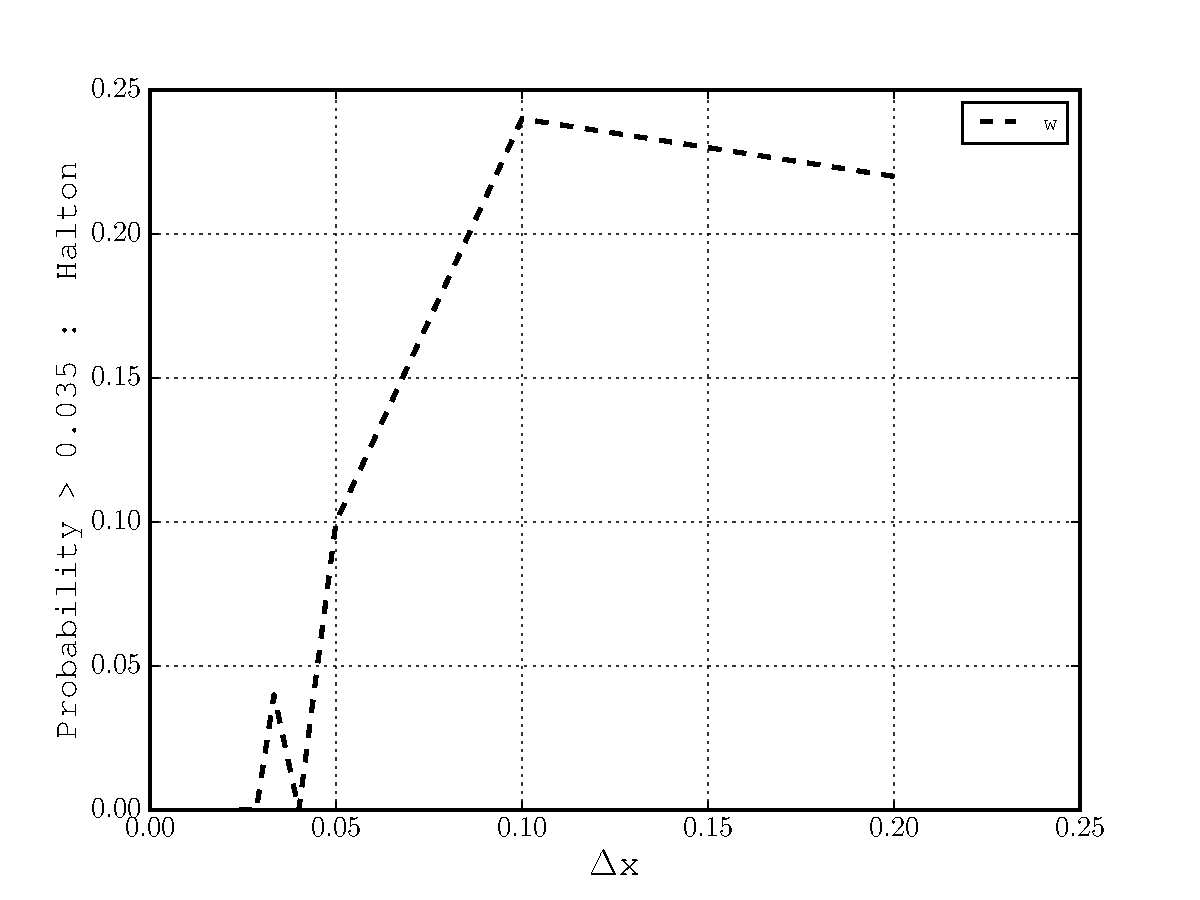
\includegraphics[width=0.77\columnwidth]{Problem4_long/Halton_wx.pdf}
  %%   \end{center}
  %% \end{figure}


  %% \begin{table}[H]
  %%   \begin{center}
  %%     \caption{Sensitivity Parameters dx = 0.1 dt = 0.5}
  %%     \begin{tabular}{l l l l l}
  %%       \toprule
  %%       Variable & Coef & Std Err & t-stat & p-value\\
  %%       \hline
  %%       $v$        &  0.1945  & 8.5335  &  0.02 & 0.9818\\
  %%       $D$        & -25.2844 & 33.3347 & -0.76 & 0.4483\\
  %%       $w$        &  76.5716 & 42.3267 & 1.81  & 0.0707\\
  %%       $\Delta t$ & -7.2201  & 1.8227  & -3.96 & 0.0001\\
  %%       $\Delta x$ &  30.8771 & 2.6986  & 11.44 & 0.0000\\
  %%       \hline
  %%       intercept & -5.1421 & 7.2558 & -0.71 & 0.4787\\
  %%       \bottomrule
  %%     \end{tabular}
  %%   \end{center}
  %% \end{table}

%\pythonscript{Problem1/Calculations}{Script for Problem}
%% \begin{figure}[H]
%%   \begin{center}
%%     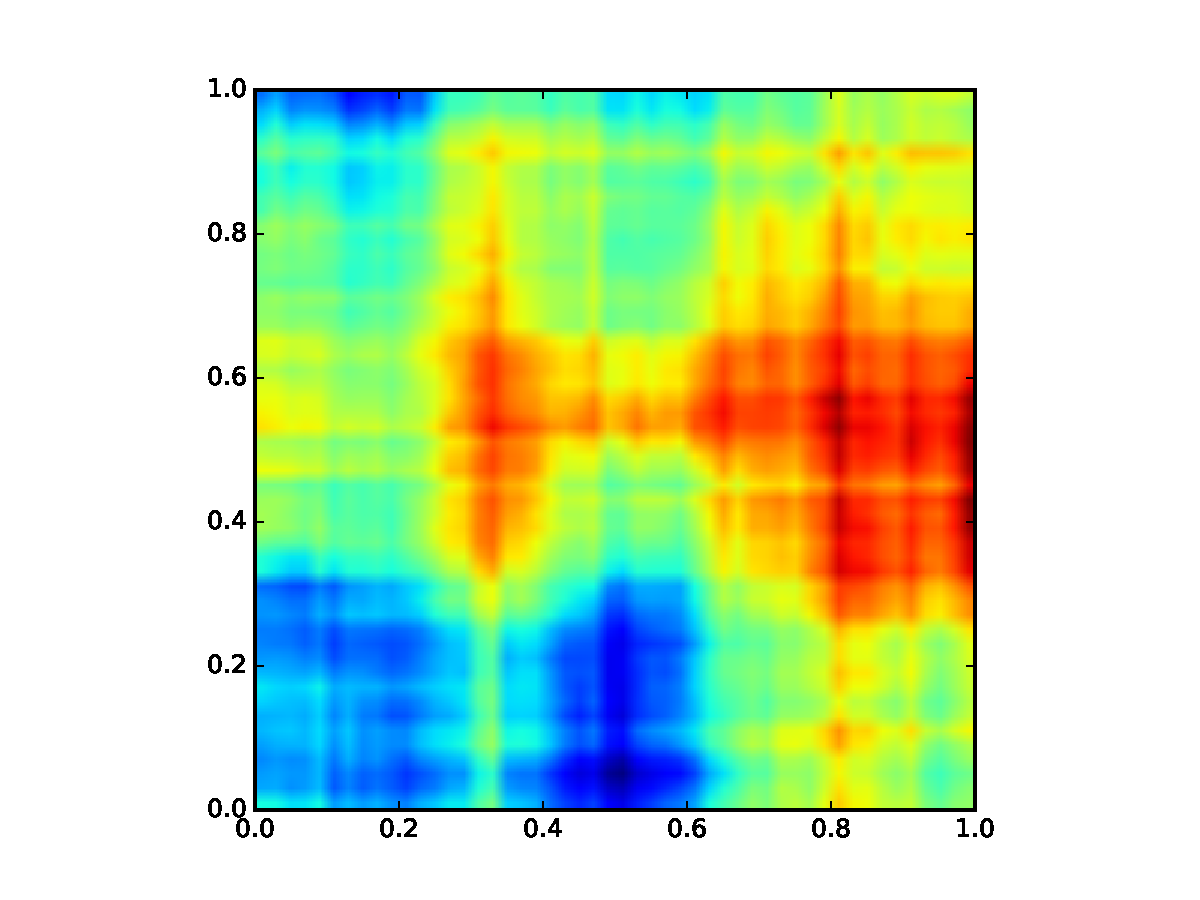
\includegraphics[width=0.77\columnwidth]{Problem1/P1realization1.pdf}
%%   \end{center}
%% \end{figure}
%\problemAnswer{TADA}

%--------------------------------------------------------------------------
%% This is an example citation \cite{Tatro2013}.
%% \bibliography{references} 
%% \bibliographystyle{plain} 

\end{document}
